% verso e anverso:
% \documentclass[12pt,openright,twoside,a4paper,english]{abntex2}
% apenas verso:	
\documentclass[12pt,oneside,a4paper,english]{abntex2} 

\usepackage[alf]{abntex2cite}	% Citações padrão ABNT
\usepackage{listings}
\usepackage{float}
\usepackage{cmap}				% Mapear caracteres especiais no PDF
\usepackage{lmodern}			% Usa a fonte Latin Modern			
\usepackage[T1]{fontenc}		% Selecao de codigos de fonte.
\usepackage[utf8]{inputenc}		% Codificacao do documento (conversão automática dos acentos)
\usepackage{lastpage}			% Usado pela Ficha catalográfica
\usepackage{indentfirst}		% Indenta o primeiro parágrafo de cada seção.
\usepackage{color}				% Controle das cores
\usepackage{graphicx}			% Inclusão de gráficos
\usepackage{pdfpages}
\usepackage{tikz}
\usetikzlibrary{automata,positioning}
\usepackage{mathtools}

\definecolor{blue}{RGB}{41,5,195} % alterando o aspecto da cor azul

\makeatletter
\hypersetup{
    %pagebackref=true,
    pdftitle={\@title}, 
    pdfauthor={\@author},
    pdfsubject={\@title},
    pdfcreator={\imprimirpreambulo},
    pdfkeywords={Linguagens}{Compiladores}{Tradução dos Comandos}, 
    colorlinks=true,       		% false: boxed links; true: colored links
    linkcolor=blue,          	% color of internal links
    citecolor=blue,        		% color of links to bibliography
    filecolor=magenta,      		% color of file links
    urlcolor=blue,
    bookmarksdepth=4
}
\makeatother

\autor{Victor Lassance (6431325)}
\title{Relatório de Compiladores\\Segunda Prova\\Compilador de \emph{SimpPro} para \emph{RNA}}
\orientador[Professor:]{Ricardo Luis de Azevedo da Rocha}
\preambulo{Texto apresentado à Escola Politécnica da Universidade de São Paulo como requisito para a aprovação na disciplina Linguagens e Compiladores no quinto módulo acadêmico do curso de graduação em Engenharia de Computação, junto ao Departamento de Engenharia de Computação e Sistemas Digitais (PCS).}
\instituicao{%
	Universidade de São Paulo
	\par
	Escola Politécnica
	\par
	Engenharia de Computação - Curso Cooperativo}
\local{São Paulo}
\data{2013}
\tipotrabalho{PCS2056 - Linguagens e Compiladores}

\setlength{\parindent}{1.3cm} % O tamanho do parágrafo
\setlength{\parskip}{0.2cm}  % Controle do espaçamento entre um parágrafo e outro
\lstset{basicstyle=\footnotesize\ttfamily}
\makeindex

\begin{document}

\frenchspacing % Retira espaço extra obsoleto entre as frases.

\imprimirfolhaderosto

\tableofcontents

\textual

\chapter{Apresentação da linguagem \emph{SimpPro} e enunciado}
\label{chap:linguagem-simppro}
	% !TEX encoding = UTF-8 Unicode

A linguagem \emph{SimpPro} foi criada e apresentada pelo professor da disciplina com características similares a de outras linguagens. As principais linguagens herdadas pela \emph{SimpPro} foram de Prolog, na forma de declaração e busca; e Lisp, na utilização dos parêntesis para declarar predicados, cláusulas e a meta.

A linguagem Prolog é declarativa, o seu texto pode conter variáveis (identificáveis lexicamente) ou nomes e números (constantes) ao estilo LISP. O operador de definição de termos é “:-”, para uma verificação de meta o operador é “?-”. Um programa em Prolog é composto usualmente de três partes: conjuntos de fatos, conjuntos de cláusulas e conjuntos de metas. Os fatos são dados sobre os quais é possível efetuar uma busca por meio de unificação de literais. As cláusulas representam a forma como os elementos de dados são inter-relacionados, definem predicados, seu uso por outros predicados e a relação entre predicados e fatos. As metas definem que tipo de resultado é esperado, podendo ser um resultado booleano, um conjunto de valores possíveis para uma variável, etc. 

Para este exercício não será utilizada a linguagem Prolog completa, apenas um subconjunto bastante limitado e simplificado denominado \emph{SimpPro}. 

A sintaxe de SimpPro fornecida em BNF foi a seguinte: 

\lstinputlisting[frame=single,breaklines=true,morekeywords={not,or,eps},basicstyle=\tiny]{files/sintaxe.txt}

Considerando que a unificação é feita através de uma busca em base dados (cuja implementação é conhecida e acessível) e que haverá apenas uma meta por programa, cujo resultado será booleano, ou seja, cada programa retornará verdadeiro (1) ou falso (0) para a meta (que será uma cláusula completa), pede-se para construir um reconhecedor determinístico, baseado no autômato de pilha estruturado, que aceite como entrada válida um programa escrito em \emph{SimpPro}.

Além disso, deve-se construir o sistema de programação para a linguagem \emph{SimpPro}, que terá um compilador para a linguagem \emph{RNA} com um ambiente de execução e uma função de busca para a meta definida. Deve ser usado a implementação de \emph{RNA} feita em linguagem C para validar o código gerado pelo compilador, aceitando ou não a meta como inferência lógica dos fatos e das cláusulas. 

	
\chapter{Apresentação da linguagem \emph{RNA}}
\label{chap:linguagem-rna}
	% !TEX encoding = UTF-8 Unicode

A linguagem de programação \emph{RNA} apresentada pelo professor é uma linguagem esotérica e nunca utilizada para aplicações práticas, criada em 2008 e implementada em 2011 por Cyrus H.  

Ela possui 16 instruções implementadas e 3 variáveis para armazenamento de memória e processamento de dados, \emph{strg}, \emph{ptr} e \emph{memory}. Como a \emph{strg}, variável responsável por guardar o índice para acesso ao \emph{memory} tem 8 bits, só podemos acessar 256 células de 8 bits cada uma, tendo uma memória bem limitada.

A Figura~\ref{fig:expl-rna} mostra a relação das 3 variáveis.

\begin{figure}[htbp]
    \centering
    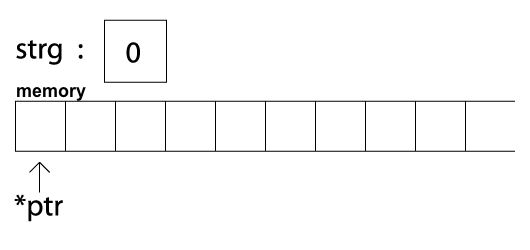
\includegraphics[width=0.6\textwidth]{./images/expl-rna.png}
    \caption{Ilustração das estruturas de armazenamento do \emph{RNA}.}
    \label{fig:expl-rna}
\end{figure}

As 16 instruções implementadas correspondem às seguintes instruções em C:

\begin{enumerate}
	\item \textbf{AUG}: \verb$int main() {$
	\item \textbf{UAA}: \verb$} // end_main$
	\item \textbf{UGG}: \verb$strg=0;$
	\item \textbf{AAA}: \verb$++strg;$
	\item \textbf{AAC}: \verb$--strg;$
	\item \textbf{GCA}: \verb$strg=*ptr;$
	\item \textbf{ACA}: \verb$ptr=&memory[strg];$
	\item \textbf{CCA}: \verb$scanf(“%d”, ptr);$
	\item \textbf{CUA}: \verb$printf(“%c”, *ptr);$
	\item \textbf{AGA}: \verb$*ptr+=memory[strg];$
	\item \textbf{AGC}: \verb$*ptr*=memory[strg];$
	\item \textbf{CAA}: \verb$*ptr-=memory[strg];$
	\item \textbf{CAC}: \verb$*ptr/=memory[strg];$
	\item \textbf{GAA}: \verb$*ptr=*ptr==memory[strg]?1:0;$
	\item \textbf{GAC}: \verb$while(*ptr) {$
	\item \textbf{UAC}: \verb$} // end_while$
\end{enumerate}

Com relação a implementação em C da linguagem\footnote{http://esolangs.org/wiki/RNA}, foram encontrados alguns erros que foram corrigidos a fim de permitir o teste de programas em RNA. Abaixo, segue o \emph{diff} do que foi modificado com relação à implementação original.

\lstinputlisting[frame=single,breaklines=true,basicstyle=\tiny]{files/diff_rna.txt}

A implementação do interpretador \emph{RNA} com as correções pode ser encontrada junto com o código final, para permitir a realização de testes.


\chapter{Analisador léxico}
\label{chap:lexico}
	% !TEX encoding = UTF-8 Unicode

Em um primeiro momento, foi definida uma linguagem de programação e identificados os tipos de átomos. Para cada átomo foi escrito uma gramática linear representativa da sua lei de formação e um reconhecedor para o átomo. Desse modo, as gramáticas assim escritas foram unidas e convertidas em um autômato finito, o qual foi transformado em um transdutor e implementado como sub-rotina, dando origem ao analisador léxico propriamente dito.

Também foi criada uma função principal para chamar o analisador léxico e possibilitar o seu teste. Cabe ressaltar que foi utilizado o analisador léxico do trabalho como base para esse, visto que a estrutura e alguns \emph{tokens} eram os mesmos. Algumas das alterações feitas para adaptar o transdutor foram:

\begin{itemize}
	\item \textbf{IDENT vs PRED + INF}: Antes, só havíamos um \emph{token} para representar identificadores de alguma forma, chamados de \textbf{IDENT}. Porém, ao observar a sintaxe do \emph{SimpPro}, foi necessário alterar o léxico para diferenciar tokens que começam com minúscula (chamado \textbf{PRED}) ou maiúscula (chamado \textbf{INF});
	\item Os operadores específicos dessa linguagem como :- e ?- foram considerados novas classes de \emph{tokens}, para facilitar a sua identificação.
\end{itemize} 

A Figura~\ref{fig:transdutor} representa o transdutor utilizado para reconhecer os \emph{tokens} da linguagem.

\begin{figure}[htbp]
    \centering
    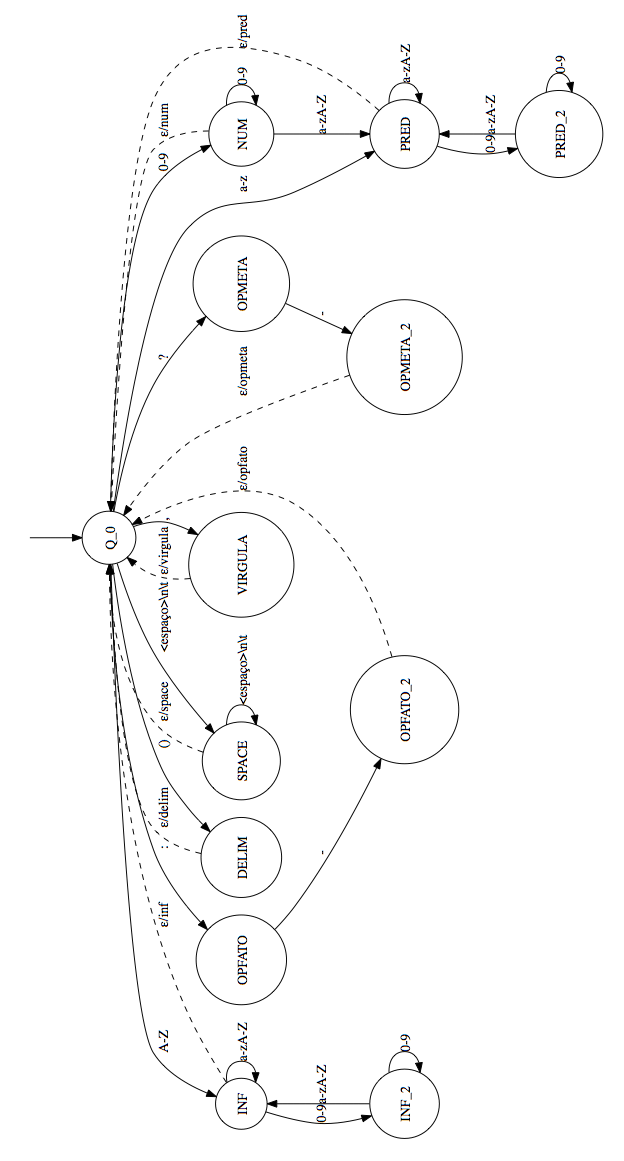
\includegraphics[width=0.7\textwidth]{./images/transdutor.png}
    \caption{Transdutor desenvolvido}
    \label{fig:transdutor}
\end{figure}

	
\chapter{Analisador sintático}
\label{chap:sintatico}
	% !TEX encoding = UTF-8 Unicode

A criação do analisador sintático, assim como com o analisador léxico, ocorreu antes da segunda prova e utilizou parte da estrutura criada para o trabalho da disciplina.

A título de recordação, o papel do analisador sintático é obter uma cadeia de tokens proveniente do analisador léxico, e verificar se a mesma pode ser gerada pela gramática da linguagem e, com isso, construir a árvore sintática. Com isso em mente, convertemos a sintaxe da linguagem \emph{SimpPro} para WIRTH, como visto abaixo.

\lstinputlisting[frame=single,breaklines=true,numbers=left]{files/WIRTHorig.txt}

A partir do WIRTH acima, reduzimos a sintaxe para conter somente um autômato, como mostrado abaixo.

\lstinputlisting[frame=single,breaklines=true,numbers=left]{files/WIRTH.txt}

Através de um script, o WIRTH gerado foi então submetido ao site do Hugo Baraúna, seu resultado salvo em arquivos locais, o JFLAP aberto automaticamente e a figura do autômato armazenada localmente, além de gerar automaticamente o pdf impresso para a primeira parte da segunda prova. A Figura~\ref{fig:automato} mostra o autômato final.

\begin{figure}[htbp]
    \centering
    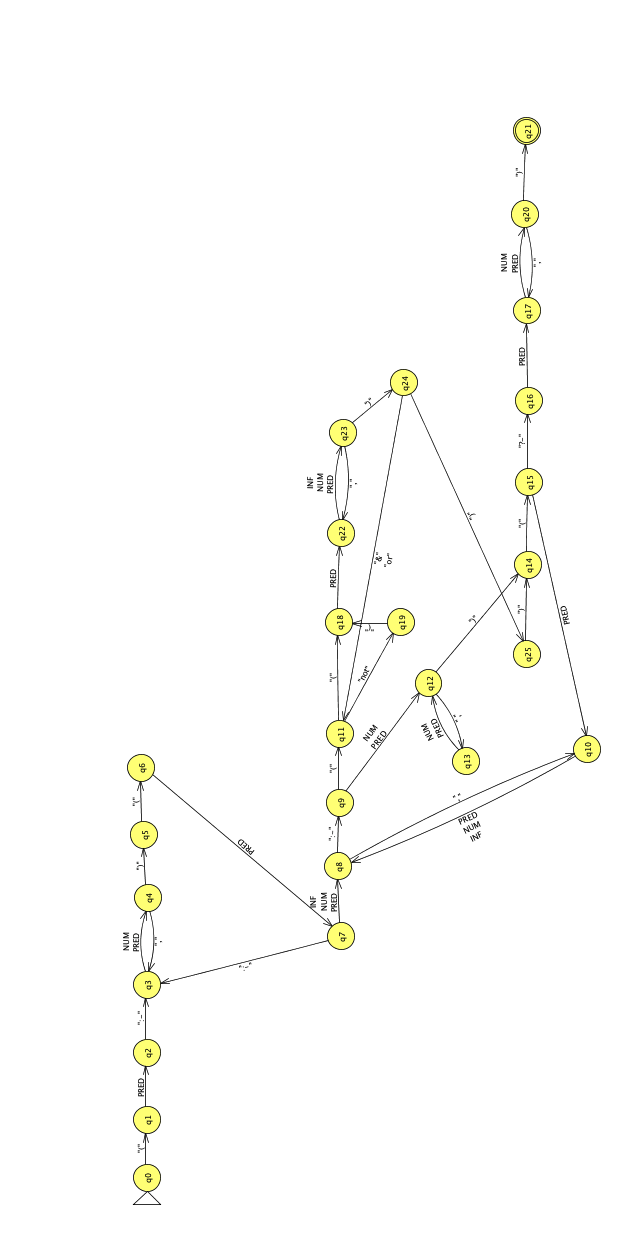
\includegraphics[width=0.75\textwidth]{./images/automato.png}
    \caption{Autômato \emph{Program}}
    \label{fig:automato}
\end{figure}


\chapter{Analisador semântico}
\label{chap:semantico}
	% !TEX encoding = UTF-8 Unicode

Durante a parte de especificação da segunda prova, a etapa 2, escolhi especificar toda a estrutura da linguagem \emph{SimpPro} dentro da memória do \emph{RNA}, com a inferência sendo executada pelo interpretador \emph{RNA}. Porém, ao observar que a variável \textbf{strg} só possuía 1 Byte, só seria possível acessar 256 células de memória, o que poderia complicar a implementação do motor de inferência no \emph{RNA}.

A partir dessa constatação, decidi implementar a geração de novos fatos a partir dos fatos originais e das cláusulas no C, de forma progressiva, sem observar a meta desejada. Com a inferência completa, foi adicionado a fita do \emph{RNA} somente a meta e a base de fatos completa, além do código que busca a meta na lista de fatos e retorna se encontrou ou não.

Foram criadas 11 ações semânticas, adicionadas no autômato em diferentes posições e exibidas na Figura~\ref{fig:semantico}.

\begin{figure}[htbp]
    \centering
    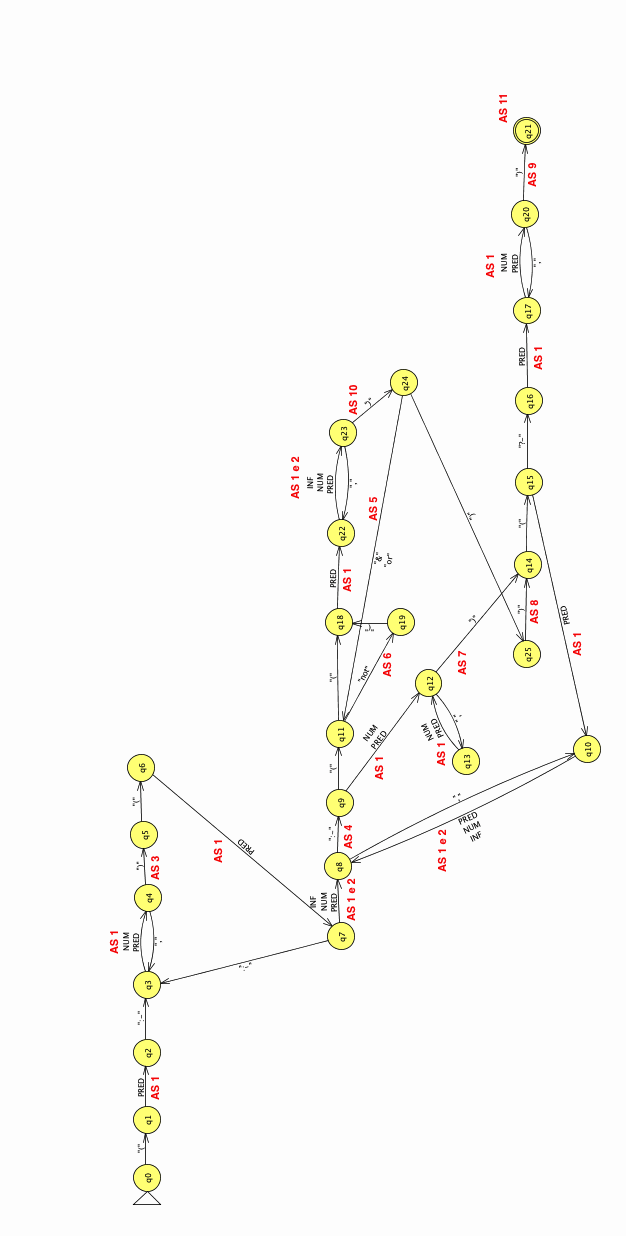
\includegraphics[width=0.75\textwidth]{./images/semantico.png}
    \caption{Autômato \emph{Program} com ações semânticas}
    \label{fig:semantico}
\end{figure}

A breve descrição das ações semânticas implementadas está listada abaixo:

\begin{enumerate}
	\item \textbf{AS 1}: Insere a constante (PRED ou NUM) na lista de constantes.
	\item \textbf{AS 2}: Insere a variável (INF) na lista de variáveis.
	\item \textbf{AS 3}: Insere o fato na lista de fatos.
	\item \textbf{AS 4}: Insere a parte esquerda da cláusula na lista de sentenças e adiciona a referência da sentença na cláusula a ser processada.
	\item \textbf{AS 5}: Insere o operador lido (``\&'' ou ``or'') na cláusula a ser processada.
	\item \textbf{AS 6}: Insere o operador not na cláusula a ser processada.
	\item \textbf{AS 7}: Ação que trata a operação (avo joao, maria :- jose, joaquim, 3), cláusulas que tem dados na parte direita da sentença. Como acordado com o professor, não será implementado por não ter correspondência com o resultado que é verdadeiro ou falso.
	\item \textbf{AS 8}: Insere a cláusula já construída nas outras ações na lista de cláusulas.
	\item \textbf{AS 9}: Insere a sentença lida como meta. Também chama o motor de inferência que gera os fatos inferidos a partir das cláusulas e dos fatos originais.
	\item \textbf{AS 10}: Insere a sentença formada previamente na lista de sentenças e adiciona a referência da sentença na cláusula a ser processada.
	\item \textbf{AS 11}: Ao terminar de ler o programa corretamente, chama a geração de código que escreve em \emph{RNA} a meta, os fatos gerados e o código necessário para verificar se a meta está contida na lista de fatos e imprimir 1 para verdadeiro ou 0 para falso.
\end{enumerate}

A geração de código foi efetuada através de uma estratégia que facilitou bastante o processo de criação dos algoritmos em \emph{RNA}. Eu desenvolvi um conversor em C++ de C para RNA e de RNA para C, utilizando a descrição dos comandos disponibilizada na Wiki da linguagem e mostrado no Capítulo~\ref{chap:linguagem-rna}. O conversor está presente no código anexado, na pasta ``rna/testes/conversor.cpp''. Com esse conversor, desenvolvi os códigos a serem gerados em C e converti ao final para \emph{RNA}, copiando o código gerado dentro do compilador. Cabe ressaltar que o conversor também foi crucial para entender e \emph{debugar} o código \emph{RNA} gerado durante o desenvolvimento.


\chapter{Realização de testes}
\label{chap:testes}
	% !TEX encoding = UTF-8 Unicode

\begin{itemize}
	\item falar sobre como testar (README e make) e como eu testei: teste compilertest e runrna
	\item relembrar a alteração no interpretador
\end{itemize}


\chapter{Exemplo de execução}
\label{chap:exemplo}
	% !TEX encoding = UTF-8 Unicode

\begin{itemize}
	\item files/simprolog.pro
	\item exemplos de execução do lextest, compilertest e runrna
\end{itemize}


\end{document}
